% coming soon

We have implemented our switching continual approach in the MAPSIM
environment~\cite{brenner:nebel:jaamas09}. Our implementation is able
to use several underlying planning systems. We have also extended the
MAPSIM system so that it can parse DTPDDL, and perform successive
estimation of the underlying belief-state using
\system{dlib-ml}~\cite{king:2009} for inference.  In this evaluation
we use our own version of Fast Downward~\cite{fast-downward} for
sequential sessions. We have extended that system to support actions
with success probabilities. In our evaluation Fast Downward is run
with the cyclic causal graph heuristic using an A* search or weighted
A* (with weight 5). We use A* for easy problems and WA* for more
difficult problems where A* is ineffective. Contingent sessions use
our own forward search procedure.


\Omit{ We then perform multiple tests with different limits for the
  belief-space size in contingent sessions.  Higher limits should
  cause longer planning times but be beneficial to plan quality as
  more contingencies can be taken in to account by the POMDP planner.
}

In order to evaluate our system, we have also implemented a baseline
approach in MAPSIM. Rather than invoking a contingent session when a
switching action $\switchAction$ is scheduled for execution, the
baseline simply executes one action that can trigger a sensing outcome
determined by the precondition of $\switchAction$, and replans in the
resulting belief-state.




%% executes switching actions and replans in the
%% resulting belief state.

%% but instead of
%% creating an observation problem for the decision theoretic planner it
%% will just execute one sensing action -- assuming that this action will
%% confirm its assumption.

To test our approach we use a robot exploration domain based on a
scenario from our physical robotic system. Here, a robot is exploring
an office or living environment, and trying to report the locations of
objects to their owner. Basic types are {\tt rooms}, {\tt places} and
{\tt objects}. Places are topological map nodes that occur in rooms.
Objects, and also the robot, are always located at a place. The robot
can move around the rooms via connections between places given by a
{\tt connected} predicate. Each room has a, possibly unknown, {\em
  category} (e.g. kitchen, office, living room). Certain objects are
more likely to be located in rooms of a particular category.  For
example, a box of cornflakes is more likely to be located in the
kitchen than the office. The robot can look for an object at a place
by executing a {\tt look-for-object} action. Executing {\tt
  look-for-object} results in a noisy sensing outcome, sometimes
indicating a positive perception if the object is there. We have that
some objects are harder to detect than others. Finally, if the robot
is in the presence of a human, it can ask what type of room it is
currently in, however conducting a dialogue is more costly than
running a vision algorithm (cost of 8 vs costs of 3).

%%  Therefore, an instantaneous positive detection of an object is
%% not proof positive of it being there.

We evaluated our switching planner against the baseline in several
tasks with the number of rooms ranging from 3 to 6. We examine the
impact of sensing reliability, experimenting using sensor models that
are: ({\em reliable}) $0.9$ chance the object is perceived if it is
present, ({\em semi-reliable}) chance is 0.65, and ({\em noisy})
chance is 0.4. The continual planning times are reported in
Figure~\ref{fig:results-time}, and the quality data in
Figure~\ref{fig:results-quality}. Here, in switching runs we examine
the performance of our system where $b_0$ allocates non-zero
probability to between 20 and 200 abstract states during contingent
sessions. For Item~$a$-$e$ the objective is to find one or more
objects and report their position to the user. In some of the tasks we
configured the environment so that no plan exists, by excluding the
desired object from the environment. Item~$f$ reports for tasks
requiring indirect sensing, where the robot must relocate to a
particular room category. For Item~$f$ there is no human in the
environment, and therefore the baseline cannot be used, because there
are no sensing schemata that directly sense room categories. In our
evaluation we run 50 simulations in each configuration, and have a
timeout on each simulation of 30 minutes (1800 seconds). In our domain,
rewards encapsulate a goal condition, and therefore we find it
intuitive to report average costs of the plans and the success rate in
problems that admit a solution (i.e., positive reward scaled by a
constant factor).

%% Because the switching utility model 

%% Using a satisficing, optimistic serial planner in sequential sessions
%% makes optimising for the expected reward difficult. Only reasoning
%% about single traces, it is optimistic wrt the remaining costs to a
%% goal and pessimistic regarding the probability of reaching it. By
%% setting the rewards to non-extremal values has little effect on that
%% system. Therefore, we do not consider expected utility in our
%% experiments. Instead, we report average costs of the plans and the
%% success rate (as a ratio between solved and solvable problems).

\begin{figure}[h!]
  % \centering
  % 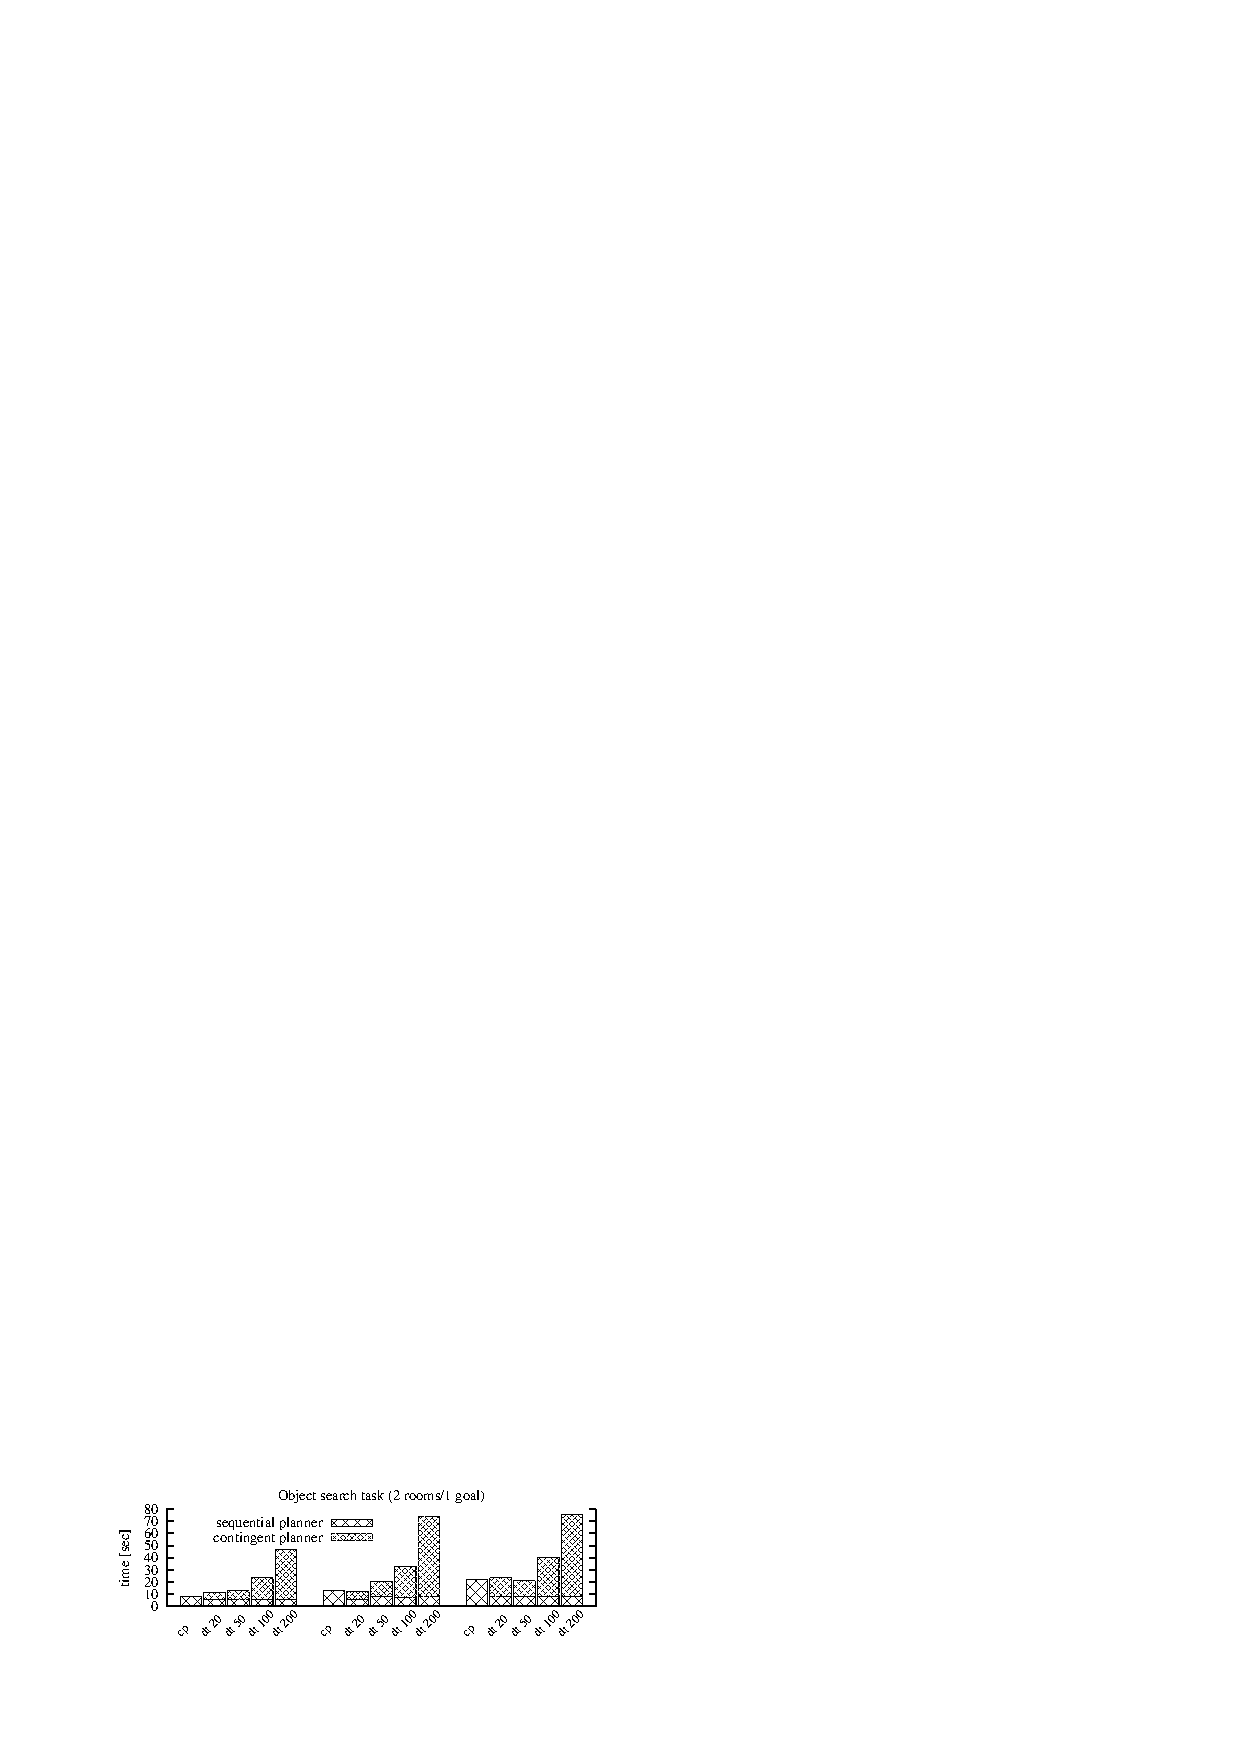
\includegraphics{dora1-time}\hfill
  % \vspace{2mm}
  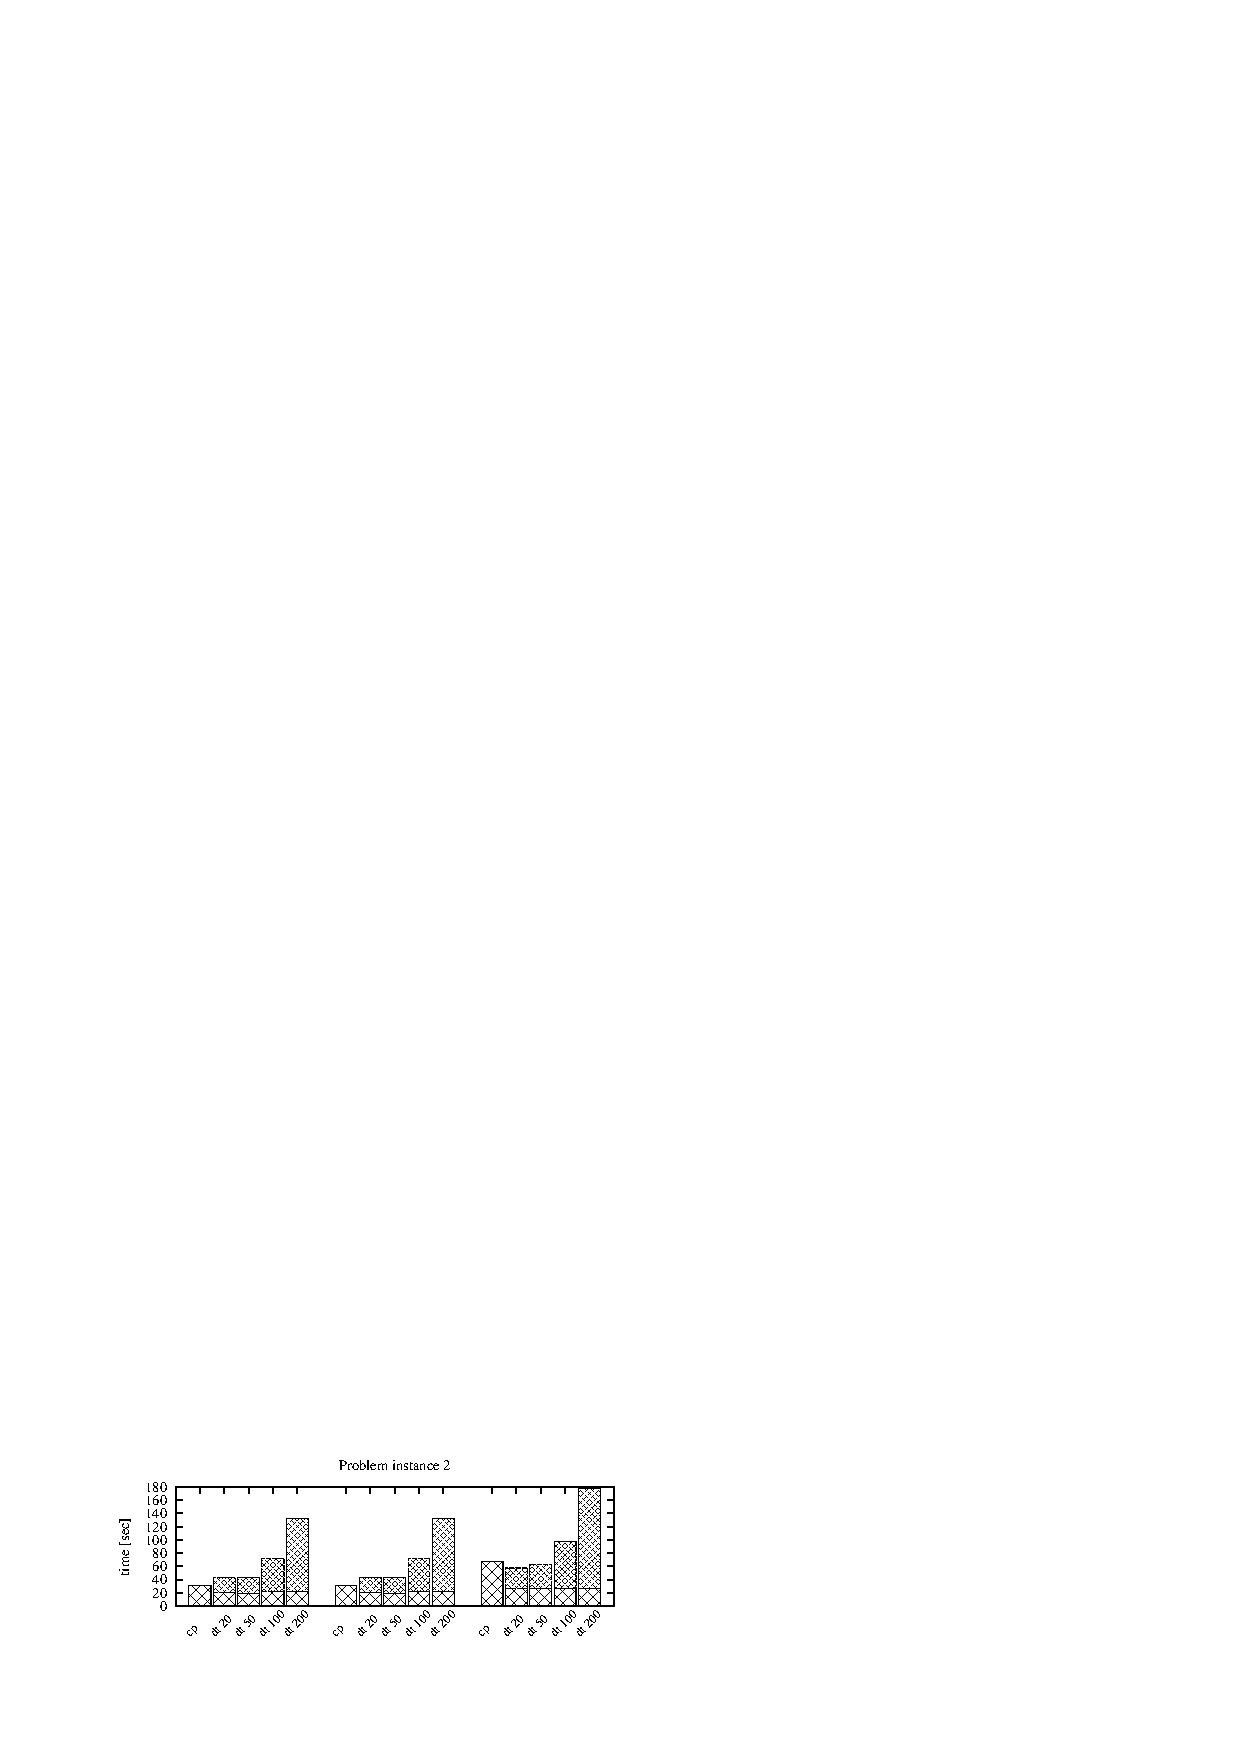
\includegraphics{dora2-time}\hfill
  % \vspace{2mm}
  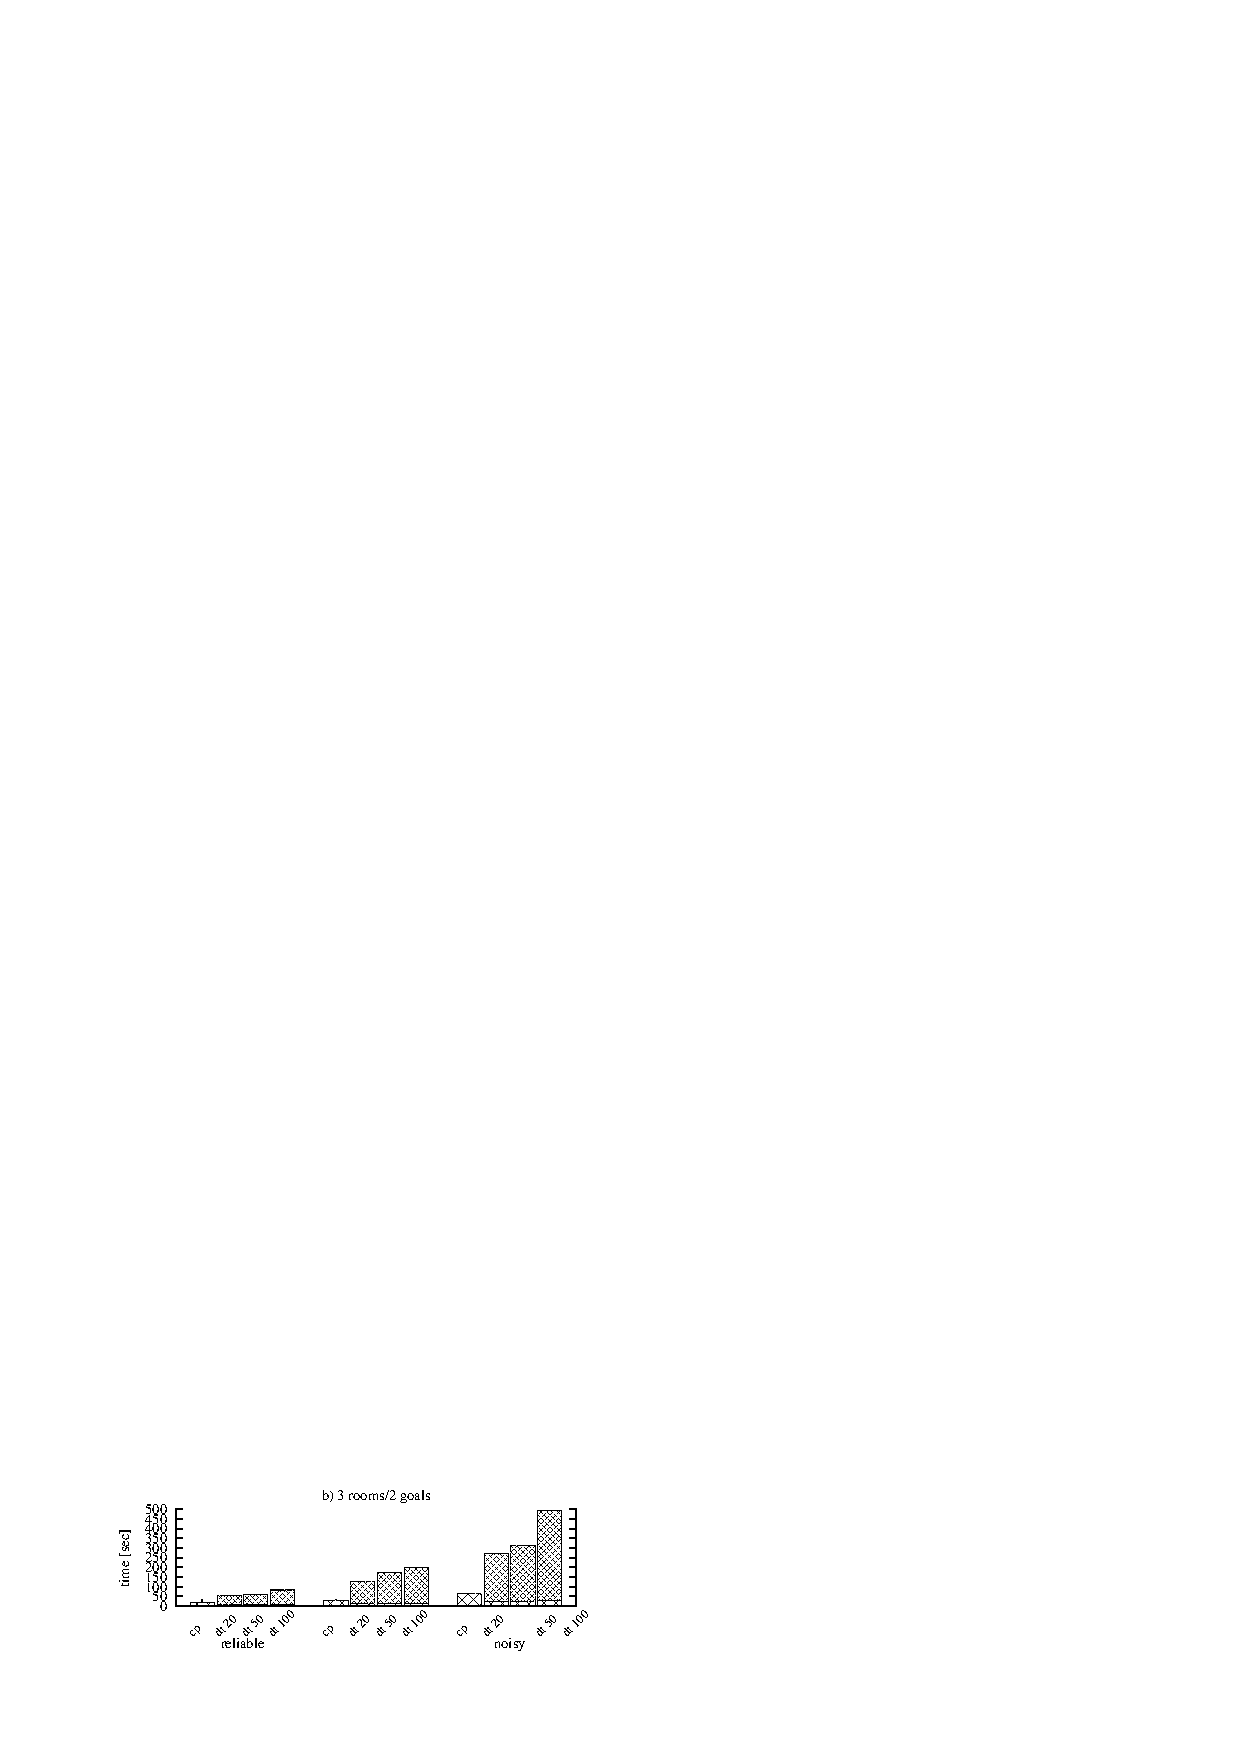
\includegraphics{dora3-time}\hfill
  % \vspace{2mm}
  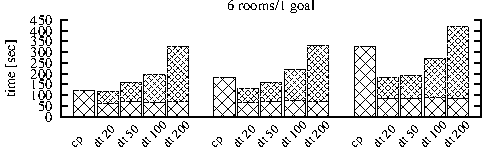
\includegraphics{dora4-time}\hfill
  \vspace{2mm}
  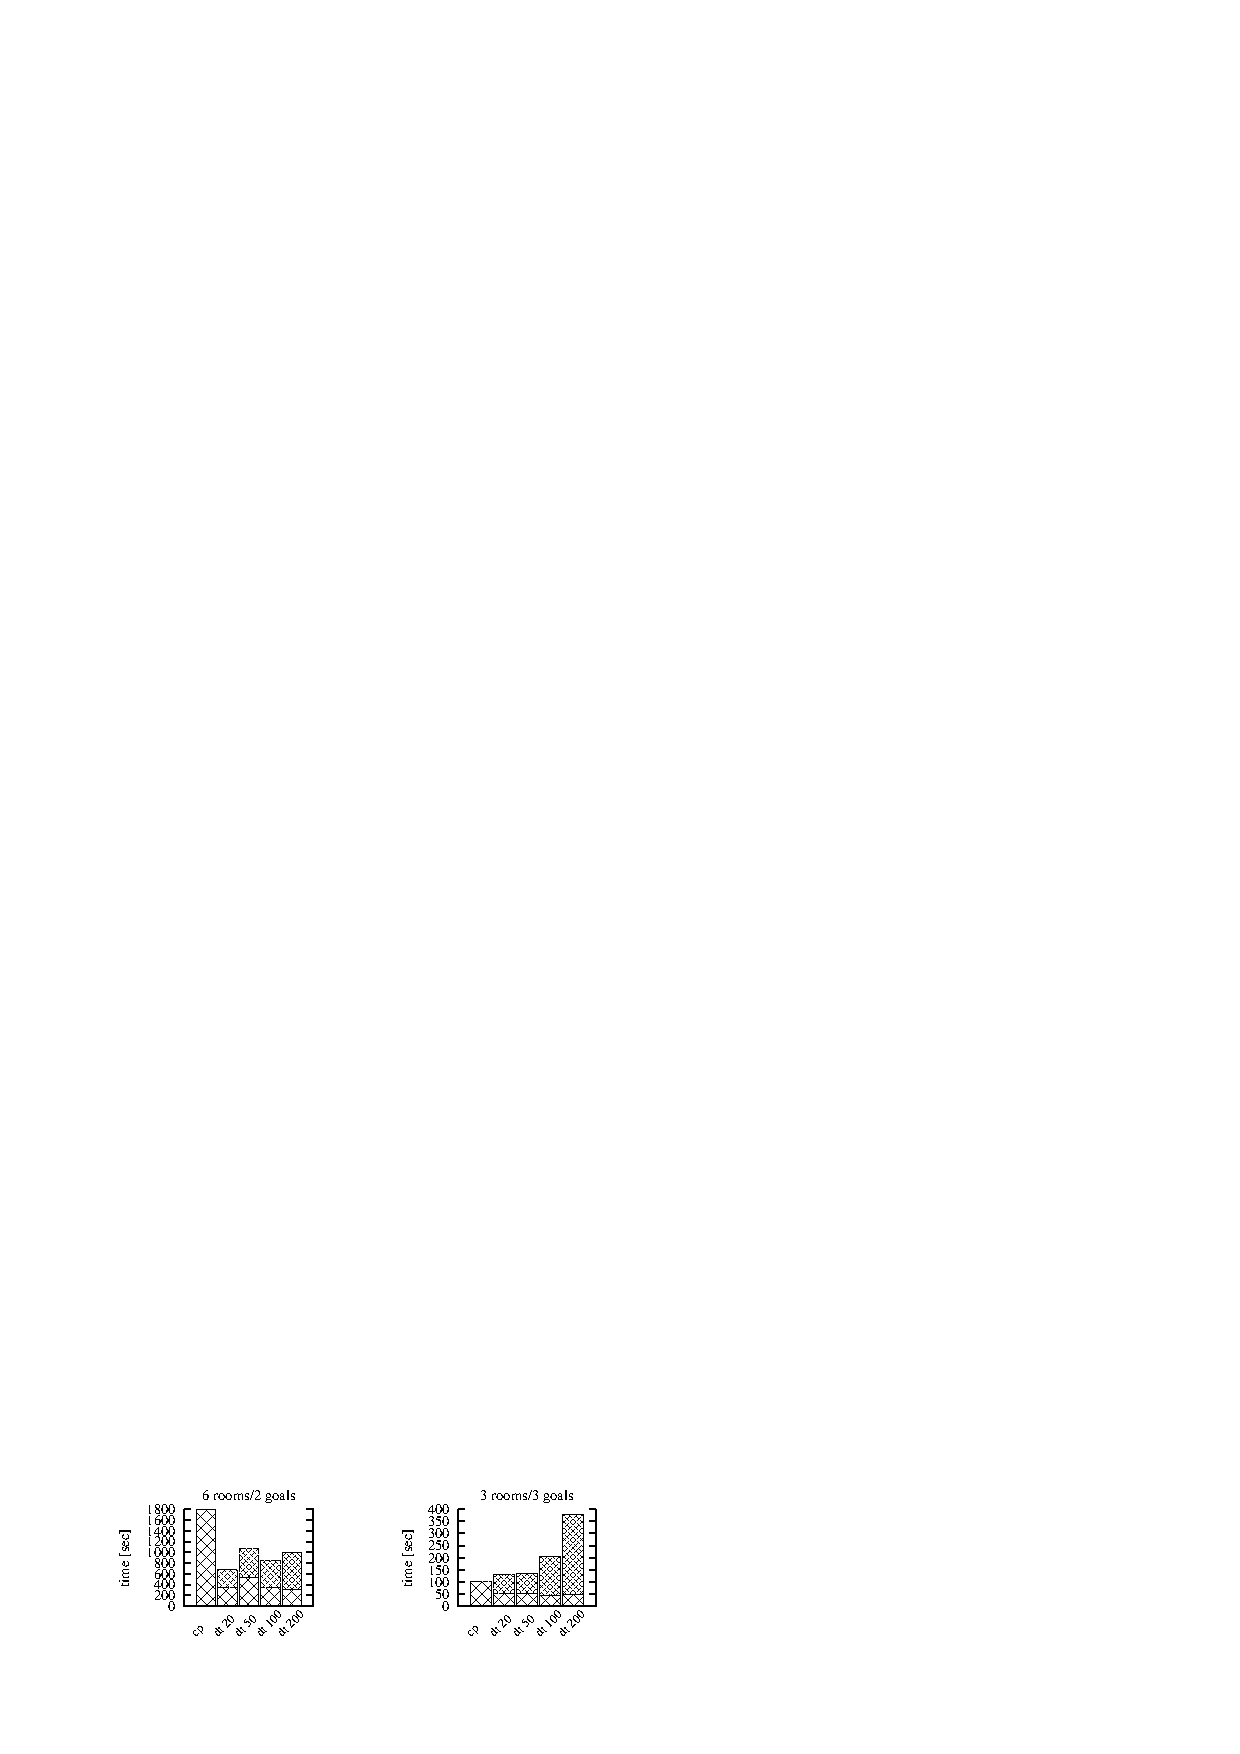
\includegraphics{dora56-time}\hfill
  \vspace{2mm}
  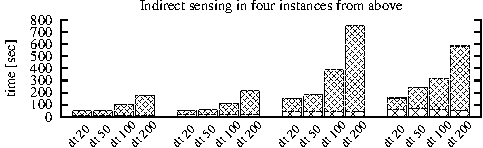
\includegraphics{dora-cat-time}\hfill
  \caption{Average runtime}
  \label{fig:results-time}
\end{figure}

\begin{figure}[h!]
  % \centering
  % 
\includegraphics{dora1-quality}\hfill
  % \vspace{2mm}
  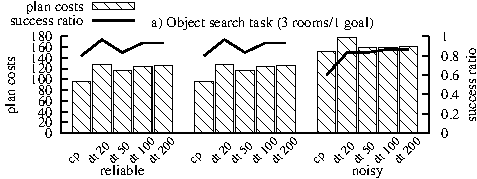
\includegraphics{dora2-quality}\hfill
  % \vspace{2mm}
  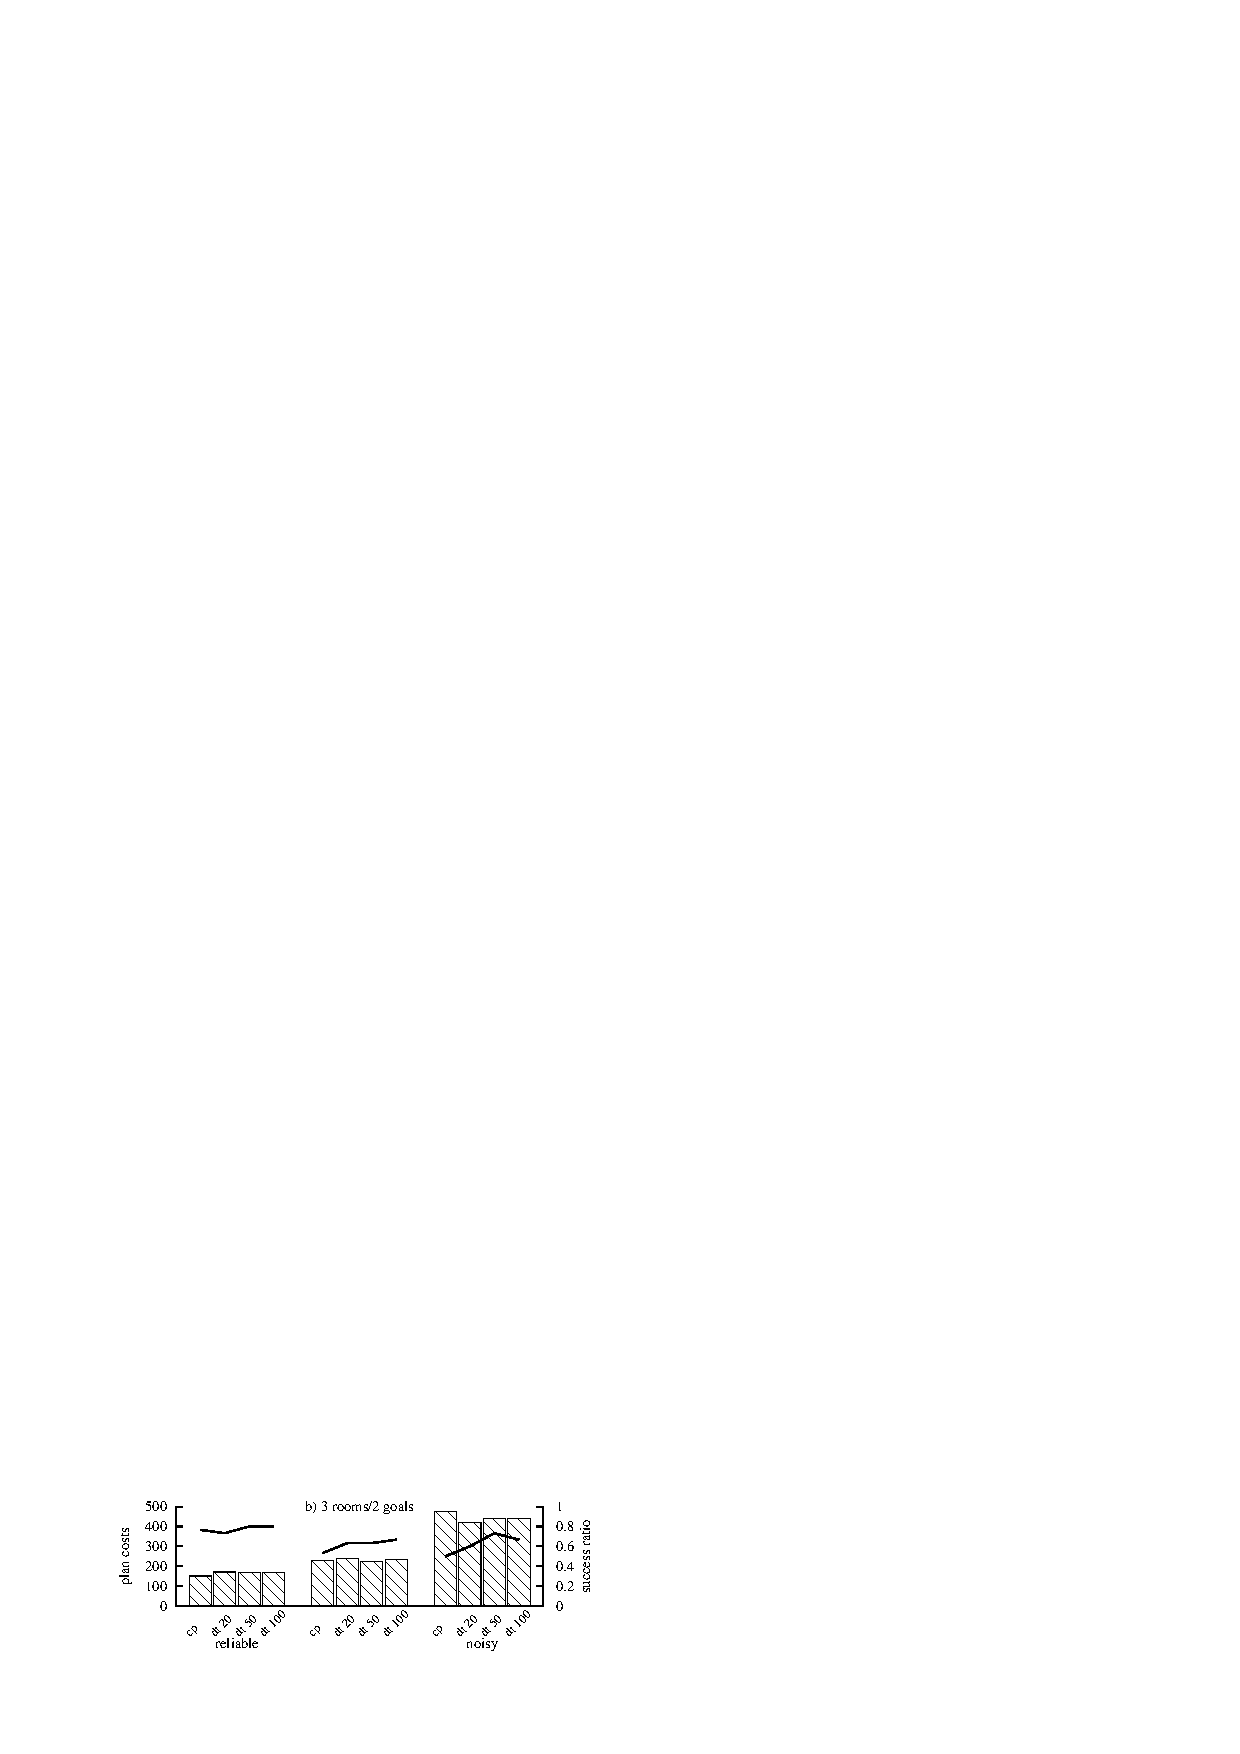
\includegraphics{dora3-quality}\hfill
  % \vspace{2mm}
  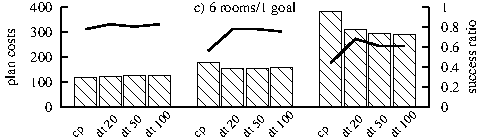
\includegraphics{dora4-quality}\hfill
  \vspace{2mm}
  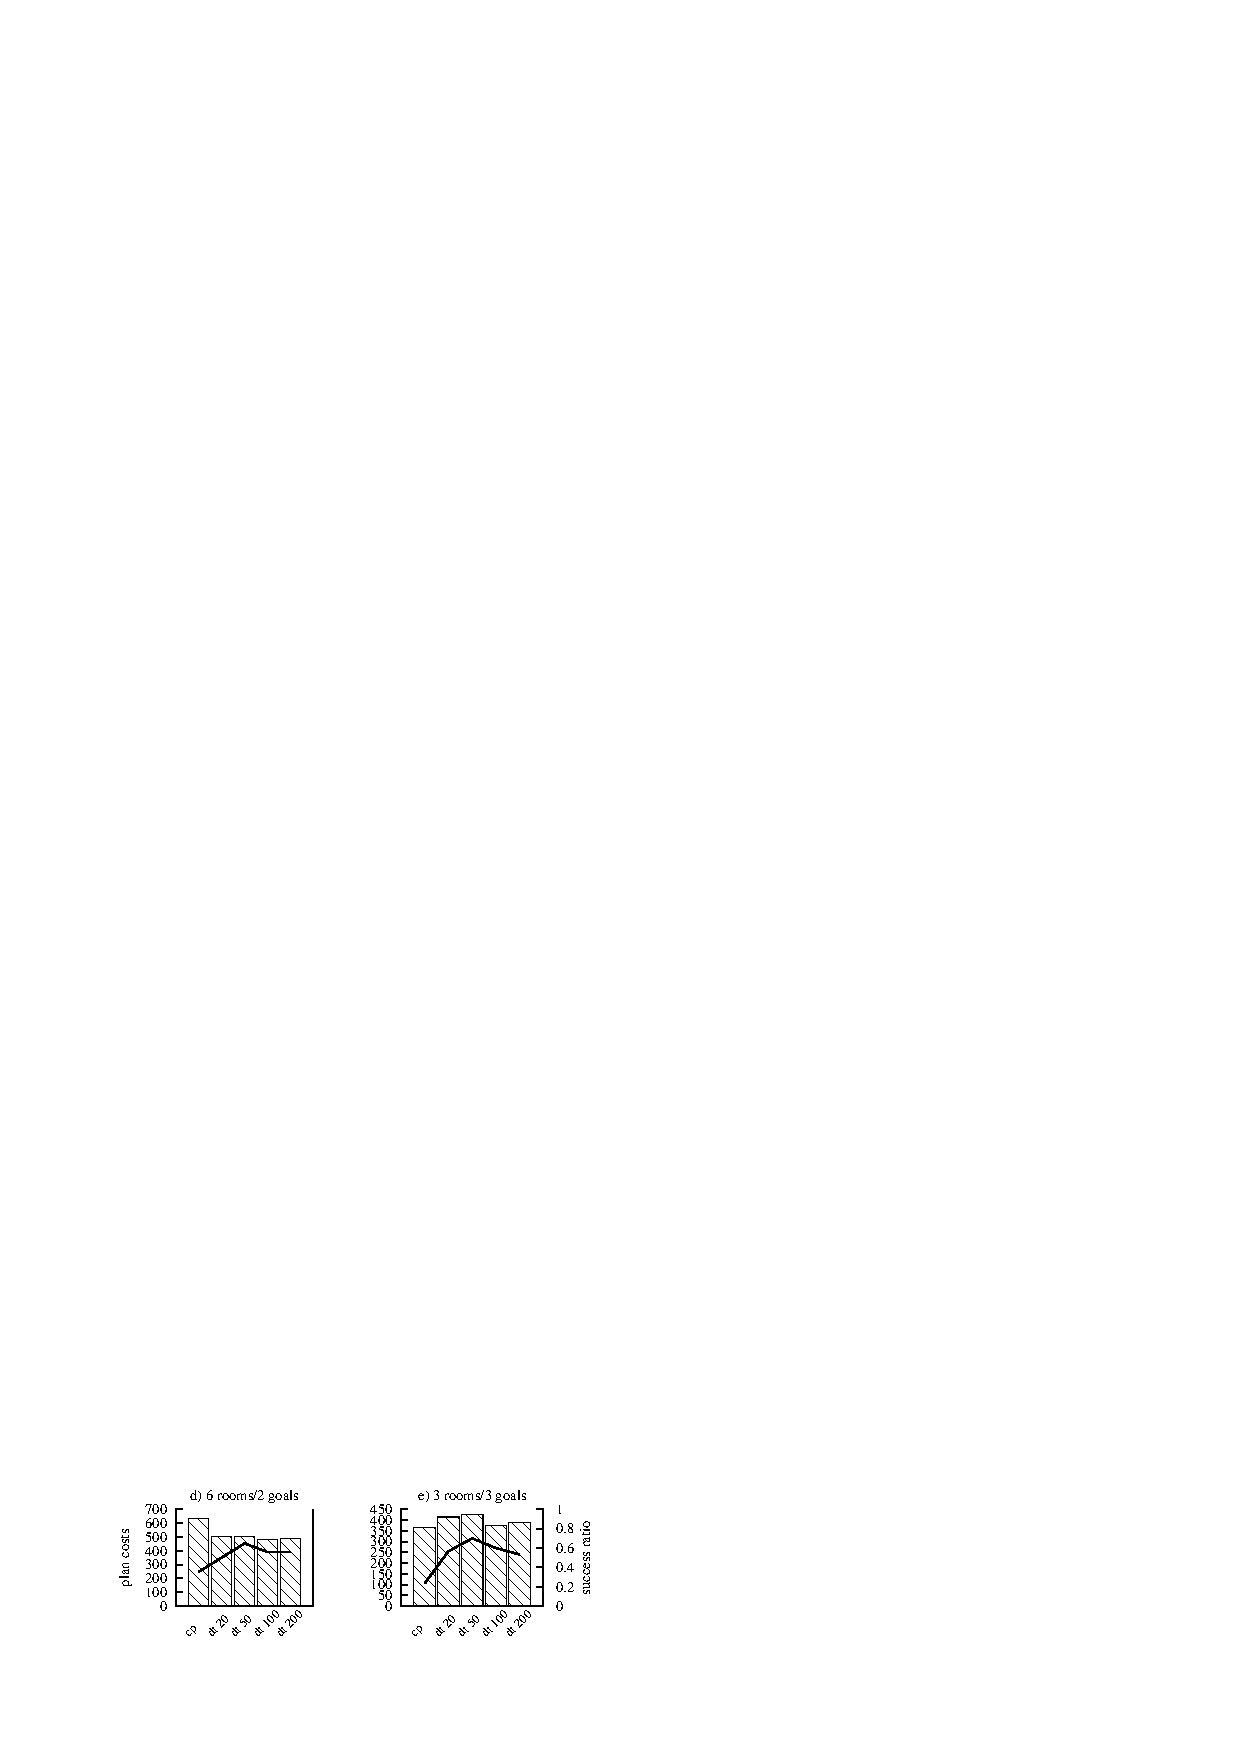
\includegraphics{dora56-quality}\hfill
  \vspace{2mm}
  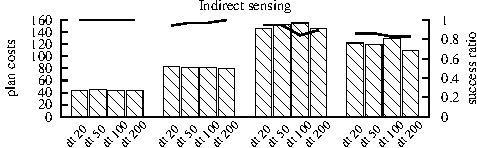
\includegraphics{dora-cat-quality}\hfill
  \caption{Average plan costs and number of successful runs.}
  \label{fig:results-quality}
\end{figure}


%% Figure \ref{fig:results-quality} shows the average costs of the
%% executed plans as well as the percentage of solvable tasks that were
%% actually solved by the planner. 

Examining success ratios and plan costs, where sensing is reliable
there is little to be gained by using the contingent planner, as the
greedy sensing approach of the baseline is sufficient. Not
surprisingly, as sensing degrades contingent planning pays off.  Also,
we find that time spent in contingent planning increases steeply as
the abstraction $\bstate_0$ becomes more refined.  That refinement
seems to be paying off in terms of the success ratio, particularly for
tasks $d$ and $e$, where we had sequential sessions using weighted
$A^*$ (rather than $A^*$). For less refined initial configurations,
the increase cost of contingent planning is compensated by a decrease
in Fast Downward planning times. The relatively high success rate
irrespective of the level of refinement in the initial configuration
indicates the effectiveness of using conditional entropy to guide
abstraction refinement in our setting.


%% :
%%while the resulting plans are still
%% longer on average, the impact on the number of solved tasks was much
%% smaller than for the baseline system.  

%% Less aggressive abstraction of the initial configuration results in
%% longer runtimes, with little to be gained in terms of plan quality. We
%% conclude that in our scenario it is worthwhile being assumptively
%% aggressive.  



%% We find that abstraction has little impact on plan
%% costs and success rate in our scenario. Increasing the size of the
%% initial abstract belief beyond 50 states rarely pays off, because
%% while additional information may facilitate better plans, the indirect
%% sensing tests report the same result. Here, we only really see an
%% impact in terms of the runtime of contingent planning.


% We believe that a part of the improvement is due to the segmentation of
% the plan into several subtask, essentially performing hierarchical
% planning. Especially when the continual planner performs badly this is
% a huge gain.

%%% Local Variables: 
%%% mode: latex
%%% TeX-master: "moritz_2011"
%%% End: 
